%! alt Convex quadrilateral ABCD with AB = 29 along the bottom, BC = 11, CD = 26 and DA = 19, and its diagonals AC and BD meeting at E. Dashed perpendiculars drop from A and C to line BD, with feet A1 and C1, and from B and D to line AC, with feet B1 and D1. The shaded quadrilateral A1B1C1D1 is a copy of ABCD turned over and shrunk by the factor 3/5, the cosine of the angle between the diagonals, so its perimeter is 51.
%! after_paragraph 1
%! scale 11/40
%! let al = 94.825800443418343093261906426008529169563801745268
% The shared preamble of every Cevian figure. pipeline/figures turns these colours into theme-aware paint,
% and refuses any other colour, so draw only with them:
%   figink (lines and labels), figaux (construction lines), figaccent (the object the argument turns on),
%   figtint and figaccenttint (light fills).
\documentclass[border=1.5pt]{standalone}
\usepackage{tkz-euclide}
\definecolor{figink}{RGB}{0,0,0}
\definecolor{figaux}{RGB}{85,85,85}
\definecolor{figaccent}{RGB}{192,57,43}
\definecolor{figtint}{RGB}{221,221,221}
\definecolor{figaccenttint}{RGB}{245,213,208}
% tkz-euclide's defaults draw circles, compasses and marks in 50% grey and fill points with a tint.
\makeatletter
\def\tkz@otherlinecolor{figink}
\def\tkz@euc@circlecolor{figink}
\def\tkz@euc@compasscolor{figink}
\def\tkz@euc@mkcolor{figink}
\def\tkz@mk@fill{figink}
\def\tkz@euc@pointfillcolor{figink}
\makeatother
\tkzSetUpLine[color=figink,line width=.7pt]
\tkzSetUpArc[color=figink,line width=.7pt]
\tkzSetUpCompass[color=figink,line width=.5pt]
\tkzSetUpPoint[color=figink,fill=figink,size=3.1pt]
\tikzset{
  every picture/.style={line cap=round,line join=round,color=figink},
  circle style/.append style={color=figink,line width=.7pt},
  aux/.style={color=figaux,line width=.45pt,dash pattern=on 2.6pt off 2pt},
  key/.style={color=figaccent,line width=1pt},
  mk/.style={color=figink,line width=.5pt},
  lbl/.style={color=figink,inner sep=2.2pt},
  len/.style={color=figink,inner sep=1.5pt,font=\small},
}

\begin{document}
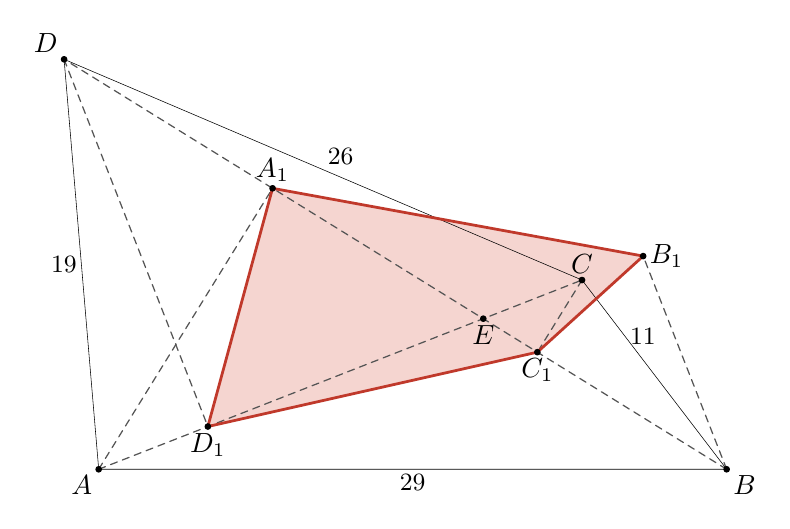
\begin{tikzpicture}
\tkzDefPoint(0.0,0.0){A} %! A = (0, 0)
\tkzDefPoint(7.9750000,0.0){B} %! B = (29, 0)
\tkzDefPoint(-0.43956127,5.2064778){D} %! D = polar(A, 19, al)
\tkzDefPoint(6.1380700,2.4033962){C} %! C = rotate(lerp(B, D, 11/dist(B, D)), B, -acos((121 + dist(B, D)**2 - 676)/(22*dist(B, D)))*180/pi)
\tkzDefPoint(4.8841846,1.9124303){E} %! E = meet(A, C, B, D)
\tkzDefPoint(2.2079116,3.5683640){Aa} %! Aa = foot(A, B, D)
\tkzDefPoint(5.5712470,1.4873130){Cc} %! Cc = foot(C, B, D)
\tkzDefPoint(6.9148447,2.7075467){Bb} %! Bb = foot(B, A, C)
\tkzDefPoint(1.3864933,0.54288933){Dd} %! Dd = foot(D, A, C)
%! fact dist(A, B) == 29
%! fact dist(B, C) == 11
%! fact dist(C, D) == 26
%! fact dist(D, A) == 19
%! fact dist(Aa, Bb) + dist(Bb, Cc) + dist(Cc, Dd) + dist(Dd, Aa) == 51
%! fact dist(Aa, Bb) / dist(A, B) == 3/5
%! fact dist(Bb, Cc) / dist(B, C) == 3/5
%! fact dist(E, Aa) / dist(E, A) == 3/5
%! fact perp(A, Aa, B, D)
%! fact perp(C, Cc, B, D)
%! fact perp(B, Bb, A, C)
%! fact perp(D, Dd, A, C)
%! fact dist(A, C) * dist(B, D) == 1725/2
%! fact area(A, B, C, D) == 345
\tkzFillPolygon[color=figaccenttint](Aa,Bb,Cc,Dd)
\tkzDrawSegments[aux](A,C B,D)
\tkzDrawSegments[aux](A,Aa C,Cc B,Bb D,Dd)
\tkzDrawPolygon(A,B,C,D)
\tkzDrawPolygon[key](Aa,Bb,Cc,Dd)
\tkzDrawPoints(A,B,C,D,E,Aa,Bb,Cc,Dd)
\tkzLabelPoint[below left,lbl](A){$A$}
\tkzLabelPoint[below right,lbl](B){$B$}
\tkzLabelPoint[above,lbl](C){$C$}
\tkzLabelPoint[above left,lbl](D){$D$}
\tkzLabelPoint[below,lbl](E){$E$}
\tkzLabelPoint[above,lbl](Aa){$A_1$}
\tkzLabelPoint[below,lbl](Cc){$C_1$}
\tkzLabelPoint[right,lbl](Bb){$B_1$}
\tkzLabelPoint[below,lbl](Dd){$D_1$}
\tkzLabelSegment[below,len](A,B){$29$}
\tkzLabelSegment[right,pos=.7,len](B,C){$11$}
\tkzLabelSegment[above right,len](C,D){$26$}
\tkzLabelSegment[left,len](D,A){$19$}
\end{tikzpicture}
\end{document}
